\section{What is Chaos?}

    \frame{\sectionpage}
    
    % \begin{frame}{The Butterfly Effect}
    %     \begin{tabular}{p{3cm}c}
    %     \begin{figure}
    %         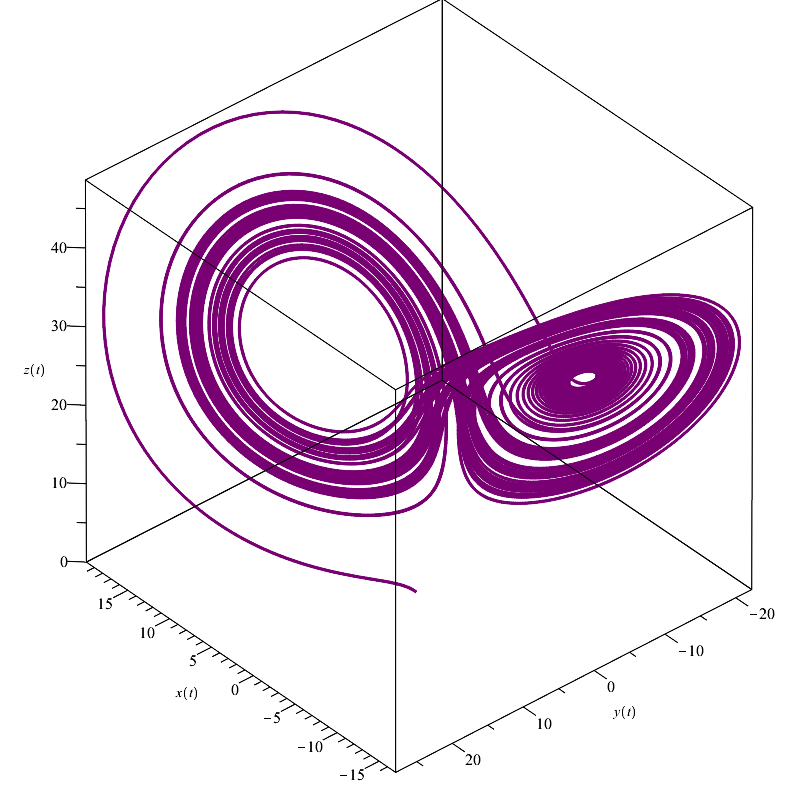
\includegraphics[width=\linewidth]{lorenz2.PNG}
    %     \end{figure}
    %     &
    %     \begin{equation}
    %         \begin{cases} 
    %         \dot{x} = \sigma(y-x) \\ 
    %         \dot{y} = rx - y - xz \\ 
    %         \dot{z} = xy - bz
    %         \end{cases}
    %     \end{equation}  
    %     \end{tabular}
    % \end{frame}       
    \begin{frame}{The Butterfly Effect}
        \begin{figure}
            \centering
            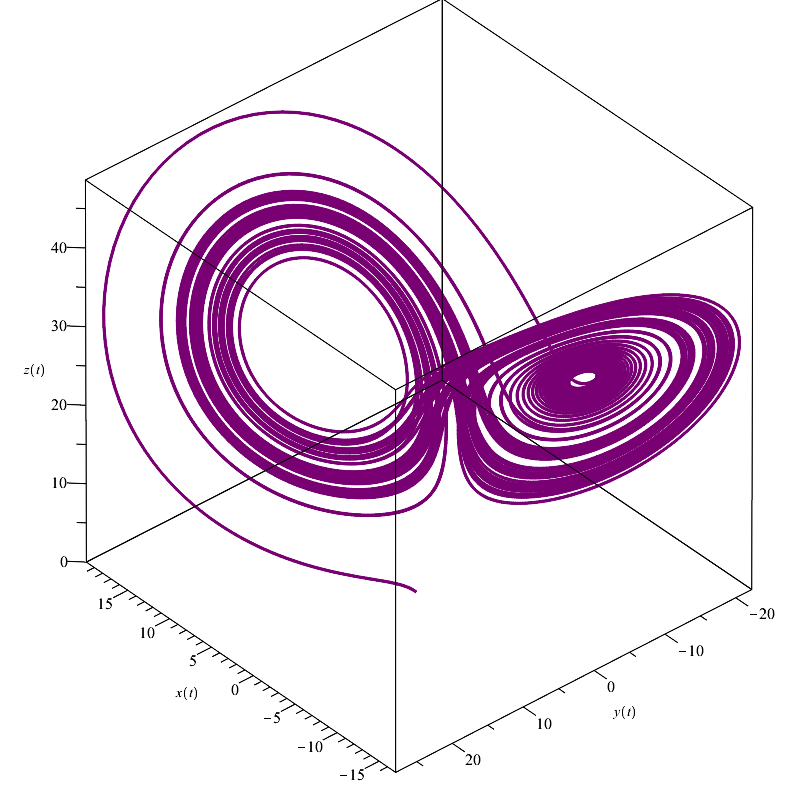
\includegraphics[height=7cm]{lorenz2.PNG}
        \end{figure}
    \end{frame}
    
    \begin{frame}{The Butterfly Effect}
        \begin{equation*}
            \centering
            \begin{cases} 
            \dot{x} = \sigma(y-x) \\ 
            \dot{y} = rx - y - xz \\ 
            \dot{z} = xy - bz
            \end{cases}
        \end{equation*} 
    \end{frame}
    
    \begin{frame}{The Butterfly Effect}
        \begin{figure}
            \centering
            \begin{figure}[ht]
                \begin{minipage}[b]{0.45\linewidth}
                    \centering
                    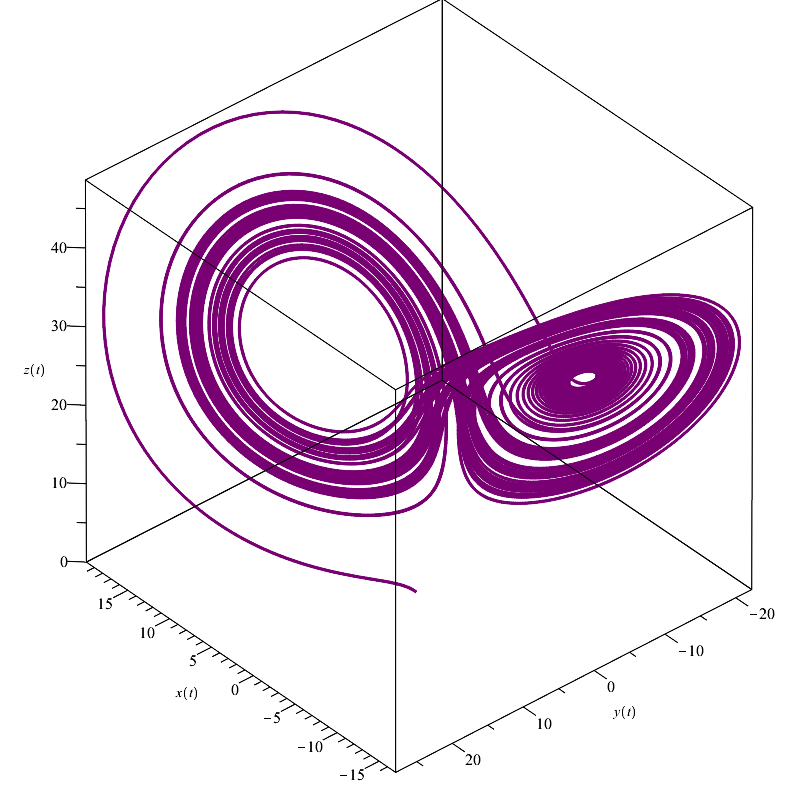
\includegraphics[width=\textwidth, height=5cm]{lorenz22.PNG}
                    \caption{chaotic, $\sigma$ = 10}
                    \label{fig:a}
                \end{minipage}
                \hspace{0.5cm}
                \begin{minipage}[b]{0.45\linewidth}
                    \centering
                    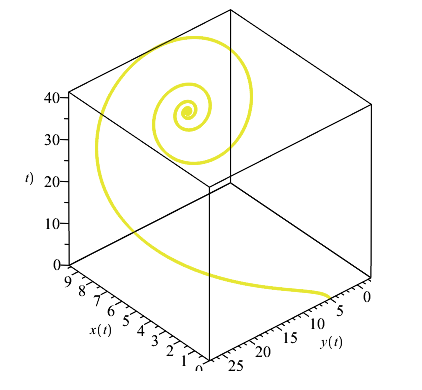
\includegraphics[width=\textwidth, height=5cm]{lorenz_s1.PNG}
                    \caption{non-chaotic, $\sigma$ = 1}
                    \label{fig:b}
                \end{minipage}
            \end{figure}
            % 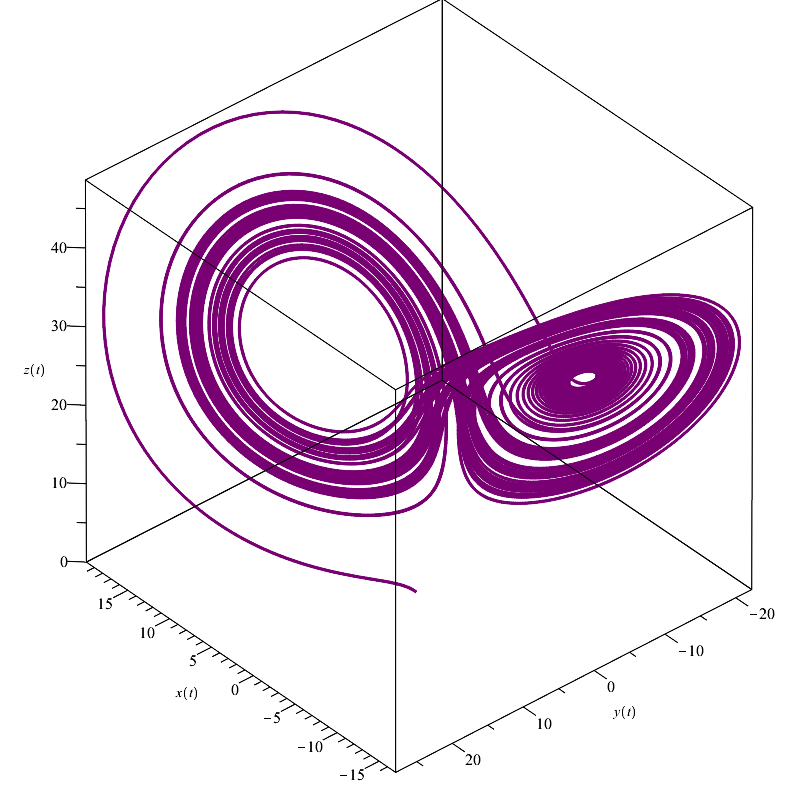
\includegraphics[width=0.6\textwidth]{lorenz2.png}%
            % 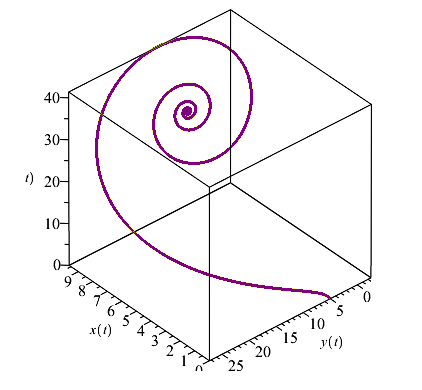
\includegraphics[width=0.4\textwidth]{lorenz_s2.png}
        \end{figure}
    \end{frame}    
    
 
 
